% !TeX program = xelatex
\documentclass{iutbscthesis}
\usepackage{comment}
\usepackage{multirow}
\usepackage{xurl}
\usepackage{rotating}
\usepackage{longtable}
% Shrink a table to the text width only when it is too wide;
% never magnify one that already fits.
\newcommand{\fitw}[1]{\resizebox{\ifdim\width>\columnwidth \columnwidth\else \width\fi}{!}{#1}}
\usepackage{fontspec}

% Bengali examples are typeset in native script. Requires XeLaTeX and the
% Nirmala UI font (ships with Windows). If compiling elsewhere, substitute any
% font with Bengali coverage, e.g. "Noto Sans Bengali".
\newfontfamily\bn{Nirmala UI}[Script=Bengali]
\newcommand{\bng}[1]{{\bn #1}}

\addbibresource{citations.bib}
% Let the bibliography stretch interword space rather than push
% long URLs past the right margin.
\AtBeginBibliography{\emergencystretch=3em}

\title{BenMedHallu: A Fact-Controlled Benchmark for Hallucination Detection in Bengali Medical Text}

\addauthor{Nashat Islam}{220041211}
\addauthor{Subha Tamanna Mrittika}{220041227}
\addauthor{Atia Zaman}{220041241}

\supervisor{Ajwad Abrar Mostofa}{Junior Lecturer}{Department of Computer Science and Engineering}
\addcosupervisor{Tareque Mohmud Chowdhury}{Assistant Professor}{Department of Computer Science and Engineering}

\department{Department of Computer Science and Engineering}
\program{BACHELOR OF SCIENCE IN COMPUTER SCIENCE AND ENGINEERING}
\defensedate{14}{September}{2026}

\begin{document}

%-------------------------- FRONT MATTER --------------------------%

\pagenumbering{roman}
\titlepage

% Declaration of candidate is mandatory per the template
\declarationofcandidate

\textbf{}
\newpage

\tableofcontents
\listoffigures
\listoftables

\clearpage

\begin{abbreviations}
    \abbr{API}{Application Programming Interface}
    \abbr{BIO}{Beginning, Inside, Outside (sequence tagging scheme)}
    \abbr{CHQ}{Consumer Health Question}
    \abbr{LLM}{Large Language Model}
    \abbr{MCQ}{Multiple Choice Question}
    \abbr{NER}{Named Entity Recognition}
    \abbr{NLP}{Natural Language Processing}
    \abbr{QA}{Question Answering}
    \abbr{Q-ALT}{Question-Alteration track of this benchmark}
    \abbr{RNG}{Random Number Generator}
\end{abbreviations}

\begin{table}[htbp]
\fitw{%
\begin{tabular}{|l|l|c|l|}
\hline
\multicolumn{1}{|c|}{\textbf{CO No.}} & \multicolumn{1}{c|}{\textbf{Course Outcome}}            & \textbf{Contributig Chapters}     &      \textbf{Marks}    \\ \hline

CO1   & \begin{tabular}[c]{@{}l@{}}Identify research problems and implement \\ innovative solutions by exploring, analyzing, \\ and applying state-of-the-art technologies, \\ frameworks, tools, and algorithms to address \\ complex real-world engineering challenges.\end{tabular} & Chapter 1, 2 and 3 & 10  \\ \hline

CO2                       & \begin{tabular}[c]{@{}l@{}}Demonstrate effective teamwork, professional\\  ethics, and responsibility by applying project \\ management principles to plan, execute, and \\ deliver a complex software system within \\ defined constraints.\end{tabular}  & Appendix A and B  & 5\\ \hline

CO3                                   & \begin{tabular}[c]{@{}l@{}}Evaluate and design computing solutions \\ considering ethical, societal, and environmental\\  implications, ensuring responsible and\\  sustainable engineering practices.\end{tabular} & Chapter 4, 5 and 7 & 10  \\ \hline

CO5                                   & \begin{tabular}[c]{@{}l@{}}Build a strong foundation for future \\ research in the same or related domains.\end{tabular}   & Chapter 8 and 9 & 5
\\ \hline

\end{tabular}%
}
\caption{Marks Distribution Summary}
\end{table}

\newpage

\begin{abstract}
Large language models increasingly answer health questions in Bengali, a language spoken by more than 230 million people but poorly served by clinical language resources. When such a model substitutes one medicine for another or softens a reported test value, the output stays fluent and confident, and nothing on the surface marks it as wrong. No benchmark measured whether a model can separate faithful Bengali medical text from corrupted text. This project builds one. Rather than annotating hallucinations found in model output, we manufacture them: authentic Bengali clinical text is edited under programmatic control, so the gold label is an output of the construction pipeline rather than a human judgement about it. The benchmark spans four task formats --- entity swapping, answer pairing, question-premise corruption, and source corruption for summarization --- yielding 19,396 labelled items and 104,502 detector judgements across six large language models. The results show a sharp asymmetry: detectors reach 94--100\% accuracy on faithful text but between 11\% and 95\% recall on corrupted text. Failure is structured, tracking both the clinical entity type swapped and the corruption operation applied, which makes the benchmark diagnostic rather than merely comparative.
\end{abstract}

%-------------------------- MAIN BODY --------------------------%
\pagenumbering{arabic}

\chapter{Introduction}

\section{Background and Motivation}

A \emph{hallucination} in natural language generation is output that is fluent and plausible but unsupported by the source or by fact \parencite{ji2023survey}. It covers two failures that behave differently under measurement: an \emph{extrinsic} hallucination asserts something the source never said, an \emph{intrinsic} one something the source contradicts \parencite{maynez2020faithfulness}.

Large language models already answer health questions for Bengali speakers, a population of more than 230 million. Here a hallucination is not a stylistic defect. A model that swaps a drug name, changes a dose, or drops a laboratory value produces text that remains grammatical, confident and recognisably clinical. The error is invisible at the surface, and the reader most exposed to it is least equipped to catch it. Three edits drawn from the benchmark built in this project, shown in \autoref{tab:motivating}, illustrate the point:

\begin{table}[H]
    \centering
    \caption{Corruptions that leave the text fluent. Each is an item from this benchmark.}
    \label{tab:motivating}
    \fitw{%
\begin{tabular}{l l l}
        \toprule
        \textbf{Original} & \textbf{Corrupted} & \textbf{Nature of the edit} \\
        \midrule
        \bng{হিস্টাসিন} & \bng{সিটিরিজিন} & A different drug of the same class \\
        \bng{৫.৯ ইঞ্চি} & \bng{৫.৯ ফুট} & The unit is rescaled \\
        \bng{রেজাল্ট পজিটিভ আসছে} & \bng{রেজাল্ট ভালো আসছে} & A specific result is generalised away \\
        \bottomrule
    \end{tabular}}
\end{table}

Bengali compounds the problem. It is low-resource for clinical NLP, with no corpus of annotated medical faithfulness judgements, and the text itself is difficult: patient messages are informal, code-mixed with English medical terms, inconsistently spelled, and often repeat one clinical detail in several paraphrases. Methods validated on English clinical notes have little purchase here. Hallucination benchmarking is nonetheless mature --- in English. TruthfulQA \parencite{lin2022truthfulqa}, HaluEval \parencite{li2023halueval} and FactCC \parencite{kryscinski2020factcc} are English resources; Med-HALT \parencite{pal2023medhalt} and MedHallu \parencite{pandit2025medhallu} add the medical domain but stay English-centric. For Bengali medical text the question had never been asked in a measurable way.

\section{Problem Statement and Objectives}

\textbf{Problem statement.} No resource measures whether large language models can distinguish faithful Bengali medical text from deliberately corrupted text, and no methodology exists for building one in which the gold label, the error type and the item difficulty are all under the builder's control.

The project pursues four objectives:

\begin{enumerate}
    \item Design a construction methodology in which hallucinated items are manufactured by applying a single named, recorded edit to authentic Bengali medical text.
    \item Instantiate that methodology across four task formats --- entity, answer, question and document level.
    \item Evaluate six large language models as detectors under one protocol, reporting accuracy by entity type, corruption operation and cost.
    \item Keep the models that generate the data and the models evaluated on it in disjoint families.
\end{enumerate}

\section{Research Challenges}

Four challenges are specific to this problem. \emph{Distribution leakage}: if hallucinated items are machine-written and faithful ones human-written, a detector can win by recognising generated prose rather than by checking facts. \emph{Label certainty}: an edit meant to remove support may fail silently, leaving an item mislabelled and penalising every detector that answers correctly. \emph{Register preservation}: patients repeat a detail in several forms, so a partial edit leaves the document contradicting itself --- a different phenomenon from the one being built. \emph{Attributable difficulty}: for a score to be diagnostic rather than merely low, exactly one experimental axis may move at a time.

\section{Contributions}

This project delivers a hallucination-detection benchmark for Bengali medical text covering four task formats and 19,396 labelled items; a construction method that derives gold labels from the pipeline and records the changed span with every item; a novel corruption operation, \emph{Coarsen}, which isolates partial support and proves the hardest condition in the benchmark; an evaluation of six detectors disaggregated by entity type, operation and cost; and a generator/detector separation that keeps the benchmark outside the self-evaluation loop prior Bengali work identifies as its own limitation.

\section{Justification as a Complex Engineering Problem}

The problem has no codified solution: constructing labelled hallucinations in a low-resource language required designing, piloting and empirically pruning six candidate corruption operations. It involves conflicting requirements, since edits must be semantically decisive yet linguistically invisible, and demands domain knowledge spanning clinical semantics, Bengali sociolinguistics and distributed system reliability. Its outcome affects public health information access for over 230 million speakers.

\section{Organisation of the Report}

\autoref{chapter:related} surveys related work and identifies three gaps. \autoref{chapter:problem} states the research questions and the scope. \autoref{chapter:proposed} presents the construction methodology and compares candidate detection approaches. \autoref{chapter:implementation} describes the system as built. \autoref{chapter:results} reports results for all four tracks. \autoref{chapter:ethics} addresses ethical, social and environmental considerations, \autoref{chapter:challenges} the challenges and limitations, and \autoref{chapter:conclusion} concludes.

\chapter{Related Works} \label{chapter:related}

\section{Two Ways to Build a Benchmark}

One family of benchmarks fixes a task, collects model output, and labels the errors that appear. TruthfulQA \parencite{lin2022truthfulqa} curates adversarial questions on which models reproduce human misconceptions; HaluEval \parencite{li2023halueval} scales this by sampling responses and filtering them through human review. Both share a structural property: the error types present are whatever the generating model happened to produce, and item difficulty is unknown to the builder. Neither can answer whether detection degrades for one corruption type rather than another, because type was never a controlled variable.

The second family manufactures errors with known properties. FactCC \parencite{kryscinski2020factcc} applies rule-based transformations to reference summaries, gaining control at the cost of transformations superficial enough for a classifier to learn the artefact rather than the semantics. \textcite{bn2025factcontrolled} go further for clinical summarization with a Leave-$N$-Out procedure on English clinical dialogue from ACI-Bench \parencite{yim2023acibench}: atomic facts are extracted from a reference, $N$ are removed from the input, and $N$ becomes an explicit difficulty dial rather than a post-hoc bin. This is the closest ancestor of the present work, though ACI-Bench holds structured English encounters whereas our corpus holds unstructured Bengali patient messages. FActScore \parencite{min2023factscore} decomposes text into atomic facts; we reuse the idea but apply it to the \emph{reference}, in order to choose what to corrupt.

\section{Medical Hallucination Beyond English}

Med-HALT \parencite{pal2023medhalt} brought hallucination testing into medicine through examination items drawn from several countries, but frames its tasks in English and treats hallucination as incorrect recall rather than unfaithfulness to a source. MedHallu \parencite{pandit2025medhallu} is closer in method to this work: it builds 10,000 medical question--answer pairs on PubMedQA, of which 1,000 are human-annotated and 9,000 deliberately generated, and stratifies them into difficulty tiers. Its finding that domain specificity amplifies the impact of hallucination motivates a medical benchmark rather than a general one, but its text is English and journal-derived, far from the informal patient register studied here.

CMHE \parencite{dou2024cmhe} is the clearest precedent for a non-English medical benchmark: 42,000 items built from Chinese medical dialogue, covering detection, diagnosis and explanation, with a portion re-verified by medical professionals. It establishes that an expert-validated medical hallucination benchmark is feasible outside English --- and, by doing so for Chinese, sharpens the absence of any equivalent for Bengali.

\section{Detection Methods and Bengali Resources}

Detection approaches divide into three. Trained entailment classifiers \parencite{kryscinski2020factcc} are cheap at inference but need labelled training data in the target language. Sampling-consistency methods such as SelfCheckGPT \parencite{manakul2023selfcheckgpt} need neither reference nor training data, detecting hallucination through disagreement across stochastic samples, at the cost of several generations per item. Zero-shot prompting of a strong model --- the LLM-as-a-judge paradigm analysed by \textcite{zheng2023judging} --- needs neither, but inherits the judge's biases. \autoref{sec:sota} returns to this choice with explicit criteria.

For Bengali the available resources are largely general-domain: BanglaBERT \parencite{bhattacharjee2022banglabert} supplies pretrained representations and XL-Sum \parencite{hasan2021xlsum} news summarization data. Two recent works are closer. BenHalluEval \parencite{adib2026benhallueval} constructs the first dedicated hallucination benchmark for Bengali, spanning question answering, code-mixed question answering, summarization and mathematical reasoning, with 12,000 hallucinated candidates evaluated under a dual-track protocol that scores ground-truth and hallucinated items separately. We adopt that dual-track protocol directly. Where BenHalluEval corrupts the \emph{summary}, the present work corrupts the \emph{source} and never edits the human summary, and it narrows the domain from general Bengali to Bengali clinical text. BanglaSummEval \parencite{banglasummeval} applies LLM judges to Bengali summarization output and explicitly names the self-reinforcing loop that arises when judge and evaluated models share a family as a limitation of its own design.

\section{Identified Gaps}

\autoref{tab:relatedworks} positions this work. The \emph{linguistic} gap: medical hallucination benchmarks exist for English and for Chinese, while the Bengali entries are general-domain. The \emph{label provenance} gap: annotation-based benchmarks label errors they encountered rather than errors they designed, leaving type, difficulty and balance uncontrolled; only the construction-based line escapes this, and it had not been applied to a low-resource language. The \emph{circularity} gap: where generator, detector and judge share a family, agreement within that family is indistinguishable from faithfulness.

\begin{table}[H]
    \centering
    \caption{Positioning of related work along task, language and label provenance}
    \label{tab:relatedworks}
    \fitw{%
\begin{tabular}{l l l l}
        \toprule
        \textbf{Work} & \textbf{Task} & \textbf{Language} & \textbf{Label provenance} \\
        \midrule
        FactCC \parencite{kryscinski2020factcc} & Summarization consistency & English & Rule-based synthesis \\
        TruthfulQA \parencite{lin2022truthfulqa} & QA truthfulness & English & Human curation \\
        HaluEval \parencite{li2023halueval} & QA, dialogue, summ. & English & Sampling + human filter \\
        FActScore \parencite{min2023factscore} & Atomic factual precision & English & Retrieval + LM validation \\
        SelfCheckGPT \parencite{manakul2023selfcheckgpt} & Detection method & English & Sampling consistency \\
        Med-HALT \parencite{pal2023medhalt} & Medical reasoning & English-centric & Exam-derived \\
        MedHallu \parencite{pandit2025medhallu} & Medical QA & English & 1k human + 9k generated \\
        CMHE \parencite{dou2024cmhe} & Medical detection & Chinese & Generated + expert re-check \\
        Leave-$N$-Out \parencite{bn2025factcontrolled} & Clinical summarization & English & By construction \\
        BenHalluEval \parencite{adib2026benhallueval} & Four tasks, general & Bengali & Generated + 3 annotators \\
        BanglaSummEval \parencite{banglasummeval} & Summarization eval. & Bengali & LLM judges \\
        \midrule
        \textbf{BenMedHallu (this work)} & \textbf{Four formats, medical} & \textbf{Bengali} & \textbf{By construction} \\
        \bottomrule
    \end{tabular}}
\end{table}

\chapter{Problem Definition and Scope} \label{chapter:problem}

\section{Problem and Research Questions}

Given a piece of Bengali medical text and its reference --- a tagged clinical entity and its sentence, a question and a proposed answer, or a source document and its human-written summary --- can a contemporary large language model determine whether the text is faithful to that reference, and on what does its ability depend? The problem is unsolved on three counts: no labelled Bengali medical faithfulness data exists, so the question cannot be asked; no construction methodology exists for such data in a low-resource setting, so the data cannot easily be made; and no protocol exists that would make a resulting score diagnostic rather than merely comparative.

\begin{description}
    \item[RQ1] Can contemporary LLMs detect entity-level hallucination in Bengali clinical text at all?
    \item[RQ2] Does detection depend on \emph{what} was corrupted --- the clinical entity type?
    \item[RQ3] Does it depend on \emph{how} --- deletion, substitution, or coarsening?
    \item[RQ4] Do model scale and price predict detection ability?
\end{description}

\section{Scope and Delimitations}

Within one semester the project builds four task formats, evaluates six detectors under one protocol, and disaggregates results by entity type, operation and cost. Explicitly out of scope: no model is fine-tuned; no hallucination mitigation or repair is attempted; no clinical validation by practising physicians is performed; only binary detection is scored, with edit spans recorded but not scored for localisation; and the summarization track is scored on its test and validation splits only.

\chapter{Proposed Methodology} \label{chapter:proposed}

\section{Overview}

The methodology rests on one inversion. Instead of generating text and labelling the hallucinations in it, we take authentic Bengali medical text known to be faithful and apply exactly one controlled, recorded edit that destroys that faithfulness. The label is an output of the pipeline rather than a judgement about it, and the record of what changed comes free. \autoref{fig:architecture} shows the complete system.

\begin{sidewaysfigure}
    \centering
    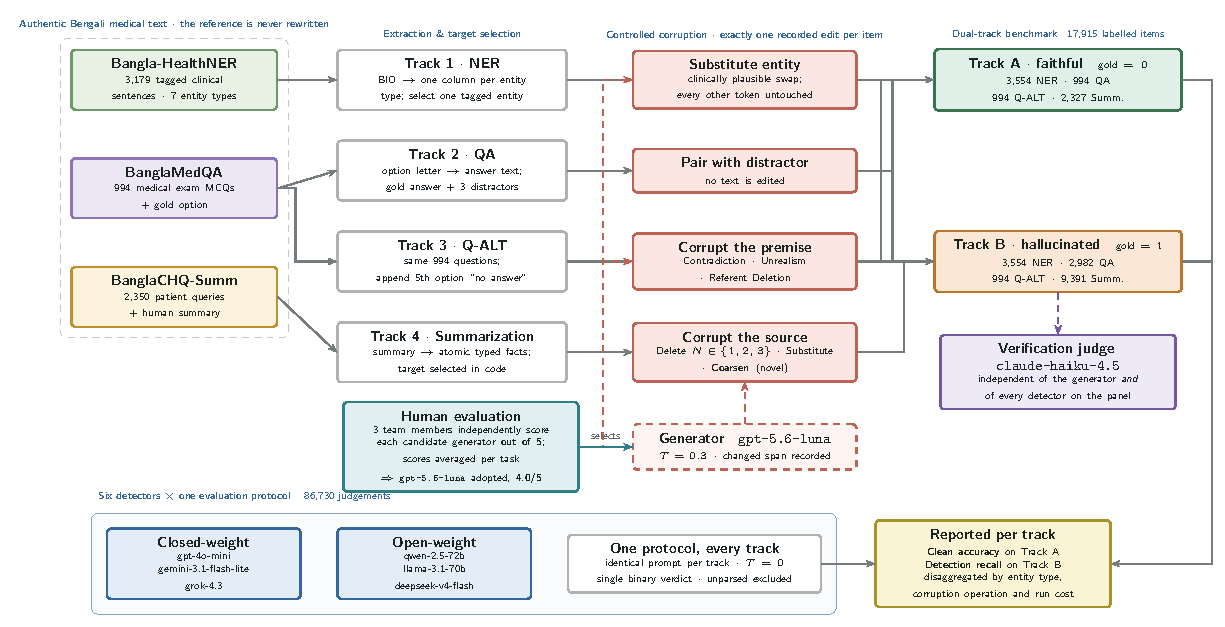
\includegraphics[width=0.96\textheight]{figures/fig_pipeline}
    \caption{End-to-end construction and evaluation pipeline. Three authentic corpora feed four tracks; each track applies exactly one recorded corruption; every item lands in Track A (faithful) or Track B (hallucinated); six detectors score every item under one protocol.}
    \label{fig:architecture}
\end{sidewaysfigure}

Three properties make later results interpretable. \emph{One text distribution}: because the edit is applied to authentic text and the reference is never rewritten, faithful and hallucinated items are drawn from the same distribution, so a detector cannot win by recognising machine-written prose. \emph{Selection in code}: the target of each edit is chosen by a seeded random number generator inside the pipeline, not by the generating model. Letting the model choose would cost the gold record of what changed, the balance across categories, and the difficulty dial, and would make two runs of the same pipeline produce different data. \emph{One axis at a time}: the deletion pipeline holds the operation fixed and varies the number of facts removed, while the alteration pipeline holds that number at one and varies the method, so a drop in accuracy is always attributable.

\section{The Four Tracks}

\textbf{Track 1 (NER)} takes a Bengali clinical sentence with tagged entities, converted from BIO tagging into one column per entity type, and replaces exactly one tagged entity with a different entity of the same class. The prompt requires the replacement to be clinically plausible, different from the original, absent elsewhere in the sentence, and to leave every other token untouched. The detector sees the sentence and the target entity and returns one binary digit. Each row is judged twice, clean and corrupted.

\textbf{Track 2 (QA)} takes a Bengali medical examination question with four options. No text is corrupted at all: the option letter is resolved to its full answer text, and the question is paired once with the correct answer and once with each of the three distractors written by the examiners. Because nothing is generated, this track acts as a control on the rest of the benchmark, and the agreement between the three distractor variants indicates whether the measurement is stable.

\textbf{Track 3 (Q-ALT)} uses the same 994 questions but corrupts the question rather than the answer. Each is rewritten so that none of options A--D can be correct, and a fifth option, \bng{``উত্তর নেই''} (``no answer''), is added. Three techniques are used. \emph{Contradiction} embeds two individually plausible but jointly impossible premises. \emph{Unrealism} states a clinically styled but factually wrong value or property. \emph{Referent Deletion} removes the essential detail behind a confident anaphoric reference whose antecedent was never supplied. Only selecting the fifth option counts as detection.

\textbf{Track 4 (Summarization)} carries the central inversion. Conventionally the source is held fixed and the summary rewritten, which makes every hallucinated summary machine-written and every faithful one human-written. Here the human summary is never edited; the \emph{source} is rewritten until it no longer supports that summary. Four stages follow: the summary is decomposed into atomic, typed facts across ten clinical categories; the target is selected in code from a seeded RNG; the generator rewrites the source so the target loses support while retained facts survive; and an independent judge verifies each fact before acceptance.

Category balance is enforced during selection. Symptom accounts for 47\% of all extracted facts, which would dominate the benchmark if sampled proportionally, so it is capped at one target per document; after the cap it accounts for 26.7\% of targets. Two categories are excluded as alteration targets on pilot evidence: Specialist, which appeared once across fifty pilot documents, and Medical Procedure, roughly half of whose instances were mislabelled in the source corpus. The Other category has identifiable spans but no swappable value slot, so it is targeted by deletion only.

\section{Selecting the Corruption Operations}

Six candidate operations were piloted on fifty documents; three shipped and three were cut, on measurement rather than judgement. The metric was \emph{claim survival}: the proportion of what the source originally said that is still present verbatim after the edit. An operation that removes nothing leaves the claim recoverable, which makes the gold label arguable. Deletion removed the most support at 21\% survival, followed by Substitute at 60\% and Coarsen at 65\%; the three cut operations left far more intact --- Reattribute 96\%, Weaken 97\% and Conflict 100\%. All three read convincingly by hand, and only the measurement exposed them.

The survivors produce three distinct support relations. \textbf{Delete $N$}, for $N \in \{1,2,3\}$, removes $N$ atomic facts, leaving claims \emph{unsupported} --- the extrinsic case. \textbf{Substitute} swaps a value for a plausible clinical neighbour, leaving the claim \emph{contradicted} --- the intrinsic case, and the arm comparable to FactCC. \textbf{Coarsen} replaces a specific value with a vaguer one that remains true of the original: where a source reported that a test kept coming back \bng{নেগেটিভ} (``negative''), the coarsened source says it kept \bng{আশানুরূপ হচ্ছে না} (``not turning out as hoped''). The summary's specific value is then unsupported while its direction of travel still is. This \emph{partial} support is isolated by no existing benchmark we are aware of, and proves the hardest case here.

The two pipelines stay separate because they compound differently. Removing three facts is a harder version of removing one, so $N$ works as a difficulty dial; altering three values at once produces a document rewritten in three unrelated ways and a failure attributable to none of them.

\section{Verification and Anti-Circularity}

Verification checks the \emph{data}; the detector evaluation measures the \emph{models}. The order matters: if a deletion silently failed and the summary is still supported, the item is labelled hallucinated, every detector correctly reports faithful, and all six are penalised for being right.

The design uses one batched call per item. The judge is shown the corrupted source together with every summary fact --- targeted and retained, shuffled so that position leaks nothing --- and returns a verdict per line. For deletion, every targeted fact must be \textsc{not\_mentioned}; for alteration, \textsc{contradicted}; for both, every retained fact must remain \textsc{supported}. The judge must be independent: not the generator, which would rubber-stamp its own edits, and not a member of the detector panel, which would make the benchmark circular.

This stage was implemented and piloted on 400 items but was not run over the full assembled dataset within the project timeline; \autoref{chapter:challenges} treats the consequence as the most significant limitation of the work. Two further filters need no model calls and were applied to the whole dataset: any item whose corrupted source came back byte-identical to the original is dropped, as is any deletion that did not shrink the document.

\section{Comparison of State-of-the-Art Approaches} \label{sec:sota}

Three established approaches could serve as the detection component; \autoref{tab:sota} compares them against the criteria that matter here.

\begin{table}[H]
    \centering
    \caption{Candidate detection approaches against project selection criteria}
    \label{tab:sota}
    \fitw{%
\begin{tabular}{l l l l}
        \toprule
        \textbf{Criterion} & \textbf{Trained classifier} & \textbf{Sampling consistency} & \textbf{Zero-shot judge} \\
        \midrule
        Bengali training data & Required & Not required & Not required \\
        Uses a reference & Yes & No & Yes \\
        Calls per item & 1 (local) & 5--20 & 1 \\
        Relative cost & Lowest & Highest & Low \\
        Cross-model comparison & Poor & Moderate & Direct \\
        Reproducibility & High & Low (stochastic) & High at $T=0$ \\
        Main weakness & No Bengali data & Proxies self-consistency & Inherits judge bias \\
        \bottomrule
    \end{tabular}}
\end{table}

The \textbf{trained classifier} is cheapest at inference and most reproducible, but is ruled out by the very gap this project exists to close: there is no labelled Bengali medical faithfulness corpus to train on, so building the benchmark is a precondition for this approach rather than an alternative to it. \textbf{Sampling consistency} needs no training data, but measures whether a model agrees with itself --- a proxy for hallucination rather than a measurement of it --- is inapplicable where a reference exists and ought to be used, and costs five to twenty generations per item.

The \textbf{zero-shot LLM judge} was adopted. The decisive criteria were that no Bengali training data is needed; that the reference is available and used; that one call per item keeps the benchmark affordable; and, most importantly for a benchmark built for comparison, that an identical prompt can be issued to every candidate model, so score differences reflect models rather than detection pipelines. Its known weakness is mitigated structurally by keeping the generating model outside the detector panel.

\chapter{Implementation} \label{chapter:implementation}

\section{Architecture and Configuration}

The repository mirrors a four-stage flow: \texttt{preprocessing/} holds the generation pipelines, \texttt{dataset/} the assembled benchmark, the \texttt{evaluation\_*} trees the raw detector runs, and aggregation scripts convert verdicts into the reported tables. Prompts and selection logic live in importable modules rather than notebooks, so that each prompt exists in exactly one place: \texttt{common.py}, \texttt{b1\_deletion.py}, \texttt{b2\_alteration.py} and \texttt{verification.py}.

Every track runs the same six stages, and only two of them differ between tracks. \autoref{tab:stages} sets them side by side.

\begin{table}[H]
    \centering
    \caption{One pipeline, four tracks. Only extraction and corruption differ; selection, filtering, evaluation and aggregation are the same code path throughout.}
    \label{tab:stages}
    \fitw{%
\begin{tabular}{@{}p{1.9cm}p{2.7cm}p{2.5cm}p{2.5cm}p{2.9cm}@{}}
        \toprule
        \textbf{Stage} & \textbf{T1 NER} & \textbf{T2 QA} & \textbf{T3 Q-ALT} & \textbf{T4 Summ.} \\
        \midrule
        1. Extract & BIO to entity columns & option letter to answer text & append a fifth option & summary to atomic typed facts \\
        2. Select & \multicolumn{4}{c}{a seeded RNG chooses the target in code, not the model} \\
        3. Generate & swap the entity & \emph{none} & rewrite the premise & rewrite the source \\
        4. Filter & \multicolumn{4}{c}{drop unchanged items; drop deletions that did not shrink the text} \\
        5. Evaluate & \multicolumn{4}{c}{six detectors, identical prompt per track, $T=0$, one binary verdict} \\
        6. Aggregate & \multicolumn{4}{c}{verdicts joined by item id into per-category and per-operation tables} \\
        \bottomrule
    \end{tabular}}
\end{table}

All models are reached through OpenRouter, an OpenAI-compatible gateway, giving one client, one retry policy and one cost ledger across six vendors. The generator is \texttt{gpt-5.6-luna}; the detectors are \texttt{gpt-4o-mini}, \texttt{gemini-3.1-flash-lite} and \texttt{grok-4.3} (closed-weight) and \texttt{qwen-2.5-72b-instruct}, \texttt{llama-3.1-70b-instruct} and \texttt{deepseek-v4-flash} (open-weight). Generation runs at temperature 0.3 and every evaluation call at 0.0. Completion-token caps are set per prompt --- three tokens on the binary NER prompt, but well above the reasoning budget on the summarization prompt, since a reasoning-capable model whose budget exceeds the cap returns an empty completion rather than an error.

\section{Source Corpora}

Three public corpora supply the authentic text, summarised in \autoref{tab:corpora}. All three are Bengali and medical, and none is rewritten at any stage.

\begin{table}[H]
    \centering
    \caption{Source corpora. The reference in each is treated as ground truth and never edited.}
    \label{tab:corpora}
    \fitw{%
\begin{tabular}{l l l}
        \toprule
        \textbf{Corpus} & \textbf{Content} & \textbf{Used for} \\
        \midrule
        Bangla-HealthNER \parencite{khan2023healthner} & tagged clinical sentences & Track 1 \\
        BanglaMedQA \parencite{sultana2025banglamedqa} & medical examination MCQs & Tracks 2 and 3 \\
        BanglaCHQ-Summ \parencite{khan2023banglachq} & patient queries with human summaries & Track 4 \\
        \bottomrule
    \end{tabular}}
\end{table}

\section{Generator Selection}

The generator choice was measured rather than assumed. Four candidate models produced corruptions for a pilot, and the three project members independently rated each candidate's output out of five for every task, with the scores averaged. \autoref{tab:genselect} gives the result. \texttt{gpt-5.6-luna} led or tied on every task and was adopted as the sole generator; the other three were not used to produce any released item.

\begin{table}[H]
    \centering
    \caption{Generator selection by human evaluation. Mean rating out of 5 over three independent reviewers.}
    \label{tab:genselect}
    \fitw{%
\begin{tabular}{l c c c c c}
        \toprule
        \textbf{Candidate generator} & \textbf{Medicine} & \textbf{Symptom} & \textbf{Health Cond.} & \textbf{Summarization} & \textbf{Mean} \\
        \midrule
        \textbf{gpt-5.6-luna} & \textbf{4.0} & \textbf{4.0} & \textbf{4.0} & \textbf{4.0} & \textbf{4.00} \\
        deepseek-v4-pro & 4.0 & 4.0 & 3.5 & 3.0 & 3.63 \\
        claude-opus-4.6 & 3.0 & 4.0 & 3.5 & 3.5 & 3.50 \\
        qwen-3.8-max & 3.5 & 3.0 & 3.0 & 3.5 & 3.25 \\
        \bottomrule
    \end{tabular}}
\end{table}

\section{Determinism and Reliability}

Selection is seeded per document, so reruns are reproducible and targets at $N{=}2$ are a strict superset of the $N{=}1$ target for the same document, making a change in accuracy attributable to the facts added rather than to a different draw.

Runs against six commercial APIs at tens of thousands of calls fail constantly, and four mechanisms were required to complete them. Results are checkpointed every fifty rows and every run resumes from its own output file, so an interruption never recomputes completed work. Multiple API keys rotate on HTTP 402 and 429. A repair pass re-runs only those rows whose stored response matches a connection-error pattern or whose verdict is null. A pre-flight probe issues one call per detector before committing a full run, a safeguard added after a reasoning model silently returned empty completions for a batch.

\section{The Resulting Benchmark}

\autoref{tab:inventory} gives the assembled benchmark. Judgement counts are actual rather than nominal: every item is judged by all six detectors, and NER items are judged twice, once clean and once corrupted.

\begin{table}[H]
    \centering
    \caption{Benchmark inventory. NER pairs are judged twice, clean and corrupted.}
    \label{tab:inventory}
    \fitw{%
\begin{tabular}{l l r r}
        \toprule
        \textbf{Track} & \textbf{Source material} & \textbf{Labelled items} & \textbf{Judgements} \\
        \midrule
        NER & 4,660 tagged clinical sentences & 5,035 pairs & 60,420 \\
        QA & 994 medical exam questions & 3,976 pairs & 23,856 \\
        Q-ALT & The same 994 questions, rewritten & 994 items & 5,964 \\
        Summarization & 2,327 messages with human summaries & 9,391 items & 14,262 \\
        \midrule
        \textbf{Total} & & \textbf{19,396} & \textbf{104,502} \\
        \bottomrule
    \end{tabular}}
\end{table}

The summarization corpus splits 1,858 / 234 / 235 across train, validation and test, and corruption yields 9,391 accepted items: Substitute 2,305, Delete $N{=}1$ 2,240, Delete $N{=}2$ 1,942, Coarsen 1,465 and Delete $N{=}3$ 1,439. The NER test set covers seven entity types, of which six were evaluated: Medicine (1,058 sentences), Specialist (650), Health Condition (577), Age (532), Dosage (495) and Medical Procedure (242). Symptom, at 1,481 sentences the largest, reached generation only.

\chapter{Results and Discussion} \label{chapter:results}

All results use temperature 0.0 and one prompt per track, issued identically to each detector. NER items are judged in pairs, so a detector's clean and corrupted figures are computed over the same underlying text. The summarization track covers the test and validation splits, giving 2,377 items per detector. Unparseable verdicts are excluded from the denominator rather than defaulted to a value. Throughout, \emph{clean accuracy} means accuracy on the faithful member of a pair and \emph{recall} the proportion of corrupted items correctly flagged; the gap between them is the principal finding of this project.

\section{Overview}

\autoref{fig:overview} places every detector on every track.

\begin{figure}[H]
    \centering
    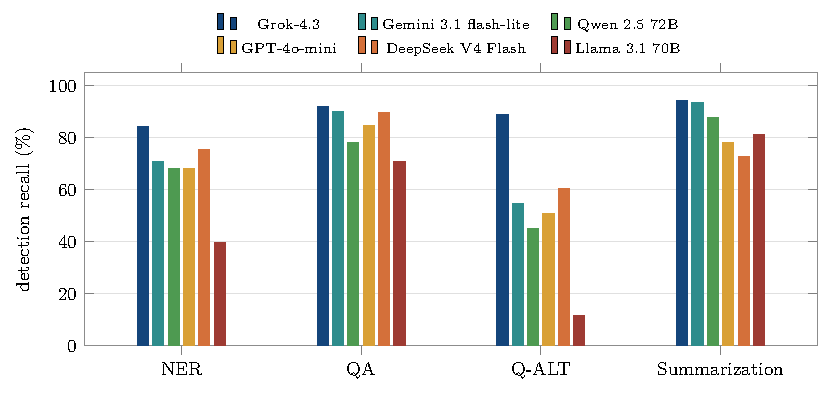
\includegraphics[width=\linewidth]{figures/fig_results}
    \caption{Detection recall by track and detector. The NER bar is the mean over its seven entity types.}
    \label{fig:overview}
\end{figure}

Two observations hold immediately. The ranking is stable: Grok-4.3 leads all four tracks and Llama 3.1 70B is last on all four, a consistency across very different task formats that is itself a result. And Q-ALT is the hardest track, with four of six detectors below 61\%. Against these figures, clean accuracy sits between 94\% and 100\% for almost every detector and category, which locates the difficulty in detection rather than in reading Bengali.

\section{Track 1: Entity-Level Detection}

\autoref{tab:nercat} reports detection recall for all seven entity types.

\begin{table}[H]
    \centering
    \caption{Track 1 detection recall (\%) by entity type, with per-detector and per-category means.}
    \label{tab:nercat}
    \fitw{%
    \begin{tabular}{l r r r r r r r r}
        \toprule
        \textbf{Detector} & \textbf{Age} & \textbf{Dosage} & \textbf{Medicine} & \textbf{Specialist} & \textbf{Health C.} & \textbf{Med. Proc.} & \textbf{Symptom} & \textbf{Mean} \\
                          & \small $n$=532 & \small $n$=495 & \small $n$=1058 & \small $n$=650 & \small $n$=577 & \small $n$=242 & \small $n$=1481 & \\
        \midrule
        Grok-4.3              & 99.2 & \textbf{97.4} & \textbf{94.7} & \textbf{83.5} & \textbf{69.2} & \textbf{73.6} & \textbf{72.5} & \textbf{84.3} \\
        DeepSeek V4 Flash     & 97.4 & 83.0 & 79.6 & 80.2 & 68.5 & 51.2 & 67.2 & 75.3 \\
        Gemini 3.1 flash-lite & 97.9 & 87.3 & 75.3 & 64.9 & 57.0 & 62.0 & 51.9 & 70.9 \\
        Qwen 2.5 72B          & \textbf{99.6} & 81.0 & 69.9 & 72.3 & 67.9 & 55.8 & 30.9 & 68.2 \\
        GPT-4o-mini           & 94.7 & 82.2 & 73.3 & 64.6 & 61.7 & 53.7 & 46.3 & 68.1 \\
        Llama 3.1 70B         & 73.1 & 50.9 & 54.4 & 15.9 & 22.7 & 31.8 & 28.9 & 39.7 \\
        \midrule
        \textbf{Category mean} & \textbf{93.7} & \textbf{80.3} & \textbf{74.5} & \textbf{63.6} & \textbf{57.8} & \textbf{54.7} & \textbf{49.6} & \\
        \bottomrule
    \end{tabular}}
\end{table}

Entity type strongly predicts difficulty, answering RQ2 affirmatively. The category means fall monotonically from Age at 93.7\% to Symptom at 49.6\%, and the division is interpretable. Age and Dosage are close to solved because the corrupted value is a \emph{number}, and a number that does not fit its context is visible without clinical knowledge. Specialist, Health Condition and Medical Procedure require knowing medicine: substituting a pulmonologist for a cardiologist is wrong only to a reader who knows what those words denote.

Clean accuracy runs between 93.9\% and 100\% for every detector and category with two exceptions, both on Medicine: DeepSeek V4 Flash at 76.7\% and Llama 3.1 70B at 79.8\%. DeepSeek is therefore the one detector whose recall on Medicine (79.6\%) exceeds its clean accuracy, meaning it over-reports rather than under-reports.

The Llama row deserves separate comment. At 15.9\% on Specialist it accepts five of every six swapped entities, while scoring 93.9\% on the matching clean sentences. A model that performs near ceiling on one half of a pair and near floor on the other is not failing to read Bengali; it is agreeing with whatever the prompt proposes. The same pattern recurs, more starkly, in Track 3.

\section{Track 2: Answer-Level Detection}

\begin{table}[H]
    \centering
    \caption{Track 2 results (\%). Wrong-answer recall is the mean over three distractor variants, which agree to within about three points.}
    \label{tab:qa}
    \fitw{%
\begin{tabular}{l r r}
        \toprule
        \textbf{Detector} & \textbf{Accepts correct answer} & \textbf{Rejects wrong answer} \\
        \midrule
        Grok-4.3              & \textbf{86.3} & \textbf{92.2} \\
        Gemini 3.1 flash-lite & 86.1 & 90.0 \\
        DeepSeek V4 Flash     & 81.0 & 89.6 \\
        GPT-4o-mini           & 66.9 & 84.7 \\
        Qwen 2.5 72B          & 67.2 & 78.2 \\
        Llama 3.1 70B         & 71.1 & 70.8 \\
        \bottomrule
    \end{tabular}}
\end{table}

\autoref{tab:qa} reports both halves of the pairing. The measurement is stable: the three distractor variants agree to within roughly three percentage points, so the ranking is not an artefact of which distractor was drawn. More interestingly, the bias direction reverses relative to Track 1. There the models under-flag, accepting corrupted text; here they over-flag. GPT-4o-mini rejects a third of the medically correct answers while still catching 84.7\% of the wrong ones, and Qwen behaves the same way. One model therefore carries two opposite failure modes depending only on framing, which is the clearest evidence for building four task formats rather than one.

\section{Track 3: Question-Level Detection}

Track 3 asks a model not to answer but to refuse, and is the hardest track in the benchmark. \autoref{tab:qalttech} breaks the results down by corruption technique.

\begin{table}[H]
    \centering
    \caption{Track 3 detection rate (\%) by technique. Items: Contradiction 436, Referent Deletion 472, Unrealism 86.}
    \label{tab:qalttech}
    \fitw{%
\begin{tabular}{l r r r r}
        \toprule
        \textbf{Detector} & \textbf{Contradiction} & \textbf{Unrealism} & \textbf{Referent Deletion} & \textbf{Overall} \\
        \midrule
        Grok-4.3              & \textbf{95.0} & \textbf{91.9} & \textbf{82.6} & \textbf{88.8} \\
        DeepSeek V4 Flash     & 72.0 & 76.7 & 47.0 & 60.6 \\
        Gemini 3.1 flash-lite & 62.4 & 62.8 & 46.4 & 54.8 \\
        GPT-4o-mini           & 46.1 & 58.1 & 53.8 & 50.8 \\
        Qwen 2.5 72B          & 51.8 & 47.7 & 37.9 & 44.9 \\
        Llama 3.1 70B         & 8.3 & 14.0 & 13.8 & 11.4 \\
        \midrule
        \textbf{Mean}         & \textbf{55.9} & \textbf{58.5} & \textbf{46.9} & \\
        \bottomrule
    \end{tabular}}
\end{table}

Technique matters as much as model. Referent Deletion is the hardest technique on average, 9 points below Contradiction and 12 below Unrealism, and it is the hardest technique individually for four of the six detectors. The explanation is structural: Contradiction and Unrealism both put something \emph{false} into the question, which sufficient clinical knowledge can catch, whereas Referent Deletion puts nothing false in at all. It removes something, leaving a confident reference with no antecedent, and detecting an absence is a materially different operation from checking what is present.

Llama 3.1 70B selected one of options A--D on 878 of 994 questions in which no such option could be correct. This is the same failure seen in Track 1 in its most extreme form: the model is not evaluating the question against its options but completing the pattern the prompt suggests.

\section{Track 4: Document-Level Detection}

\begin{table}[H]
    \centering
    \caption{Track 4 overall results (\%) and measured run cost over 2,377 items per detector.}
    \label{tab:summ}
    \fitw{%
\begin{tabular}{l r r r r}
        \toprule
        \textbf{Detector} & \textbf{Clean} & \textbf{Corrupted} & \textbf{Overall} & \textbf{Run cost (USD)} \\
        \midrule
        Grok-4.3              & 89.1 & \textbf{94.2} & \textbf{93.2} & 4.567 \\
        Gemini 3.1 flash-lite & 89.3 & 93.5 & 92.6 & \textbf{0.137} \\
        Qwen 2.5 72B          & 89.6 & 87.8 & 88.1 & 0.489 \\
        GPT-4o-mini           & \textbf{93.6} & 78.0 & 81.1 & 0.098 \\
        Llama 3.1 70B         & 78.0 & 81.1 & 80.5 & 0.697 \\
        DeepSeek V4 Flash     & 89.6 & 72.9 & 76.2 & 0.121 \\
        \bottomrule
    \end{tabular}}
\end{table}

GPT-4o-mini again inverts its Track 1 profile: best of all six on untouched pairs at 93.6\%, but only 78.0\% on corrupted sources. The cost column answers RQ4 bluntly. Grok-4.3 finishes first at 93.2\% but costs \$4.57 against \$0.137 for Gemini 3.1 flash-lite, which finishes 0.58 points behind --- a thirty-three-fold cost difference for a gap well inside the noise of a single run. Model scale fares no better as a predictor: the 70B open-weight model places last on every track it completed.

\begin{table}[H]
    \centering
    \caption{Track 4 recall (\%) by corruption operation. Deletion becomes easier as $N$ rises; Coarsen collapses.}
    \label{tab:summmethod}
    \fitw{%
\begin{tabular}{l r r r r r}
        \toprule
        \textbf{Detector} & \textbf{Del. $N{=}1$} & \textbf{Del. $N{=}2$} & \textbf{Del. $N{=}3$} & \textbf{Substitute} & \textbf{Coarsen} \\
        \midrule
        Grok-4.3              & \textbf{98.0} & \textbf{100.0} & \textbf{100.0} & \textbf{95.9} & \textbf{72.7} \\
        Gemini 3.1 flash-lite & 97.4 & \textbf{100.0} & \textbf{100.0} & 94.0 & 71.7 \\
        Qwen 2.5 72B          & 90.6 & 99.2  & 99.7  & 84.3 & 62.3 \\
        Llama 3.1 70B         & 85.3 & 92.1  & 96.0  & 72.2 & 59.3 \\
        DeepSeek V4 Flash     & 70.9 & 82.8  & 84.8  & 73.1 & 51.2 \\
        GPT-4o-mini           & 77.6 & 91.3  & 93.3  & 80.2 & 42.7 \\
        \midrule
        \textbf{Mean}         & \textbf{86.6} & \textbf{94.2} & \textbf{95.6} & \textbf{83.3} & \textbf{60.0} \\
        \bottomrule
    \end{tabular}}
\end{table}

\autoref{tab:summmethod} separates the same items by the operation applied, and two clean gradients answer RQ3. Deletion becomes \emph{easier} as $N$ rises, from 86.6\% at one fact to 95.6\% at three: more missing material means more signal, and the monotonic trend --- which holds for all six detectors individually, without exception --- confirms that $N$ works as the intended difficulty dial. Second, Coarsen collapses. At a mean of 60.0\% it sits 23 points below Substitute and 36 below Delete $N{=}3$, and GPT-4o-mini catches only 42.7\% of it, worse than chance on a binary task, which means it is systematically wrong rather than merely uncertain. The reason follows from the operation: the source still discusses the detail and still points the same way, so a detector checking for topical agreement finds it and stops.

\autoref{tab:summcat} disaggregates the same items by the category of the targeted fact.

\begin{table}[H]
    \centering
    \caption{Track 4 recall (\%) by targeted fact category, across the six detectors.}
    \label{tab:summcat}
    \fitw{%
\begin{tabular}{l r r r}
        \toprule
        \textbf{Fact category} & \textbf{Best} & \textbf{Worst} & \textbf{Mean} \\
        \midrule
        Medicine          & 98.1 & 79.1 & \textbf{90.7} \\
        Other             & 98.7 & 81.1 & 90.6 \\
        Dosage            & 100.0 & 68.8 & 90.3 \\
        Health Condition  & 98.1 & 78.9 & 90.2 \\
        Age               & 100.0 & 76.5 & 89.6 \\
        Symptom           & 96.7 & 74.6 & 85.9 \\
        Test Result       & 87.4 & 70.4 & 79.9 \\
        Temporal          & 88.8 & 66.1 & 78.1 \\
        \bottomrule
    \end{tabular}}
\end{table}

Temporal and Test Result are the two hardest categories, and they are precisely the categories in which Coarsen applies most naturally: a date or a laboratory value can be made vaguer without being made false, whereas a medicine name largely cannot. The category result and the operation result are therefore two views of the same mechanism.

\section{Qualitative Examples}

\autoref{tab:examples} gives one item per corruption type, with the number of detectors that flagged it. These are drawn across the difficulty range rather than selected to favour the benchmark.

\begin{table}[H]
    \centering
    \caption{Representative items and how many of the detectors caught each.}
    \label{tab:examples}
    \fitw{%
\begin{tabular}{@{}p{2.4cm} p{4.6cm} p{4.6cm} c@{}}
        \toprule
        \textbf{Operation} & \textbf{Original} & \textbf{Corrupted} & \textbf{Caught} \\
        \midrule
        NER, Medicine & \bng{হিস্টাসিন} & \bng{সিটিরিজিন} & 3/6 \\
        NER, Specialist & ``Heart er doctors'' & ``Pulmonologist'' & 3/6 \\
        NER, Health Cond. & \bng{বদহজম} & \bng{গ্যাস্ট্রাইটিস} & 3/6 \\
        \midrule
        Q-ALT, Unrealism & \bng{কত BMI কে স্বাভাবিক ওজন হিসেবে ধরা হয়?} & premise fixes the normal range at 20.0--24.9, so no option is correct & 1/6 \\
        \midrule
        Summ., Coarsen & \bng{বার বার নেগেটিভ হচ্ছে} & \bng{বার বার আশানুরূপ হচ্ছে না} & 0/6 \\
        Summ., Substitute & \bng{শ্বাসকষ্ট হয় কিছুটা} & \bng{মাথা ঘোরে কিছুটা} & 0/6 \\
        \bottomrule
    \end{tabular}}
\end{table}

The Medicine example is instructive: both terms are antihistamines, so the substitution is clinically plausible but wrong, and it splits the detector panel exactly in half. The Unrealism example is stronger still. The true normal BMI range begins at 18.5, which was option C of the original question; with the premise falsely fixed at 20.0--24.9, no option can be correct, yet five of six detectors selected one anyway.

\section{Cross-Track Discussion}

Five findings hold across all four tracks. \emph{The benchmark measures a real failure}: clean accuracy of 94--100\% alongside recall as low as 11\% shows the difficulty lies in detection, not in reading Bengali. A detector at ceiling on clean text and near chance on corrupted text is not a weak reader but a reader carrying a prior that the text it is shown is fine --- exactly the prior a medical deployment cannot afford. \emph{Failure is structured}, moving predictably with both entity type and operation, which is what makes the benchmark diagnostic rather than merely comparative. \emph{Bias direction is task-dependent}, reversing between Tracks 1 and 2. \emph{Scale and price are weak predictors}. And \emph{absence is harder than error}: the two hardest conditions in the benchmark, Referent Deletion and Coarsen, are both cases in which nothing stated is false.

No prior benchmark measures Bengali medical faithfulness, so direct numerical comparison is not meaningful. Two qualitative points stand. The monotonic relationship between $N$ and accuracy reproduces in Bengali the behaviour \textcite{bn2025factcontrolled} report for English clinical dialogue, which is evidence that fact-controlled construction transfers across languages and registers. And the Substitute arm shared with FactCC \parencite{kryscinski2020factcc} is \emph{not} the hardest condition here --- Coarsen is 23 points harder --- so a benchmark restricted to substitution would have overstated how well current models handle unfaithfulness.

\chapter{Ethical, Social, and Environmental Considerations} \label{chapter:ethics}

\textbf{Ethical Aspects.} The corpora are Bengali patient messages and publicly available examination questions. Because patient messages can carry identifying detail, no personally identifying information is introduced, reconstructed or inferred at any stage; the pipelines edit clinical facts only, and prompts forbid adding information beyond what the edit requires. Prior work whose methods we adapt \parencite{bn2025factcontrolled, kryscinski2020factcc, adib2026benhallueval} is cited at the point of adaptation, so that the boundary between borrowed and original method is unambiguous. A second consideration is specific to this project: its output is, by construction, a corpus of plausible-looking but medically wrong Bengali clinical text, which carries misuse potential if mistaken for genuine advice. It is therefore released with every item explicitly labelled, the corrupted span recorded and the operation named. The benchmark is a measuring instrument and must not be used as a source of medical information.

\textbf{Social Aspects.} Hallucination benchmarks are overwhelmingly English, so the assurance that a deployed model behaves safely is far weaker for a Bengali speaker than for an English one, even when the same model serves both. Making Bengali medical faithfulness measurable supplies evidence a deployer would need before putting such a system in front of patients, and the results argue for caution: a model that accepts five of six swapped clinical entities is not fit for unsupervised health advice. That a low-cost model matches a frontier model here also carries an equity implication --- adequate safety checking need not be restricted to organisations that can afford frontier inference.

\textbf{Environmental Aspects.} Evaluating six models over roughly 86,700 API calls has a real energy cost, reduced deliberately. Token caps were set per prompt, in one case to three tokens; checkpointing and resume mean an interrupted run never recomputes completed work; and the faithful pair in Track 4 is deduplicated by document rather than scored once per variant, which removed 8,634 redundant calls. No model was trained or fine-tuned. The cost analysis in \autoref{tab:summ} is itself an efficiency result: a flash-tier model within 0.6 points of a frontier model at one thirty-third the cost is evidence for a lower-energy deployment choice.

\chapter{Challenges and Limitations} \label{chapter:challenges}

\section{Challenges}

\emph{API cost.} One frontier detector cost \$4.57 on a single track against \$0.10--0.14 for flash-tier models. This constrained which models could cover which tracks and was the direct cause of the coverage decisions described below.

\emph{No annotator pool.} With three project members and no external annotators, human verification could not be performed at the scale of the assembled dataset, which is why the verification stage was piloted rather than run in full.

\emph{API reliability at scale.} Credit exhaustion and rate limiting interrupted long runs constantly; key rotation, checkpointing and repair passes were built specifically to make completion possible.

\emph{Reasoning models returning empty completions.} A model whose reasoning budget exceeds the token cap returns an empty string rather than an error. Discovered only after a batch had been spent, this led to the mandatory pre-flight probe.

\emph{Designing corruptions that hold up.} Half the candidate operations did not survive the pilot, leaving 96--100\% of the claim verbatim in the source. All three read convincingly by hand; only measuring claim survival exposed them.

\section{Limitations}

\emph{Verification not applied to the released set.} This is the most significant limitation. The verification judge is implemented and was piloted on 400 items, but it was not run over the full assembled dataset within the timeline, so released items passed only the two mechanical filters. A residual proportion may carry an incorrect gold label, which would depress all six detectors' recall roughly equally; the reported \emph{rankings} are therefore more trustworthy than the absolute values.

\emph{Detection only, no mitigation.} The project measures whether models catch hallucination. It does not attempt to reduce or repair it, so the results describe a problem without yet testing a remedy.

\emph{Incomplete coverage.} In the summarization track, 7,483 corrupted items in the training split remain unscored.

\emph{No clinical validation.} All corruptions are model-generated; no clinician has confirmed that the substituted entities are plausible in context, nor that the coarsened values genuinely remove support.

\emph{Statistical treatment.} Each track uses a single prompt at temperature 0, with no prompt-sensitivity study, self-consistency sampling or significance testing. Differences of one or two points should not be treated as meaningful.

\emph{Single generator.} Every corruption in the released benchmark was produced by one model. The pilot compared four generators and found detector scores varied little between them, but the possibility of a generator-specific artefact cannot be excluded on that evidence alone.

\chapter{Conclusion and Future Work} \label{chapter:conclusion}

\section{Findings and Contributions}

\textbf{RQ1} is answered affirmatively but narrowly: frontier models can detect Bengali medical hallucination, but only Grok-4.3 does so reliably on both halves of a pair. \textbf{RQ2} affirmatively: entity type predicts difficulty, with category means falling from 93.5\% on Age to 54.7\% on Medical Procedure, the division falling cleanly between numeric and knowledge-bound types. \textbf{RQ3} affirmatively and more strongly --- the operation matters more than the entity type, with mean recall spanning 36 points from Coarsen at 60.0\% to three-fact deletion at 95.6\%. \textbf{RQ4} negatively: a 70B open-weight model places last on every track, and a flash-tier model matches a frontier reasoning model to within 0.6 points at one thirty-third the cost.

The project delivers a hallucination-detection benchmark for Bengali medical text spanning four task formats, 19,396 labelled items and 104,502 detector judgements. It shows that fact-controlled construction transfers from English clinical dialogue to informal Bengali text, contributes the Coarsen operation isolating partial support, and demonstrates a generator/detector separation that removes the self-evaluation loop prior Bengali work identifies in its own design.

\section{Future Work}

\begin{enumerate}
    \item \textbf{Extend to open-ended question answering.} Every task format in this benchmark is closed-form: entity substitution, multiple choice, multiple choice with refusal, and summarization against a fixed source. Free-form generation remains untouched, and is where hallucination is most consequential, since no option list constrains the model and no reference summary supports a direct comparison. Evaluating it requires claim-level decomposition of the generated answer followed by per-claim adjudication against the source, and is the largest remaining gap in coverage.
    \item \textbf{Diagnose the causes of failure.} The benchmark reports where detection breaks down but not why. The Coarsen result is the natural starting point: replacing a specific value with a vaguer one that remains true of the original defeats every detector tested, which suggests that models verify consistency rather than sufficiency. Whether that pattern holds across entity types, corruption depth and model scale is answerable in part from the existing data and in full with targeted probes.
    \item \textbf{Hallucination mitigation.} The natural successor to measuring detection is improving it: chain-of-thought prompting, retrieval support, and an explicit ``not sure'' option are all testable against this benchmark without new data.
    \item \textbf{Run the verification judge at scale.} The stage is written and piloted; executing it over the full dataset converts a well-filtered dataset into a verified one, and is a precondition for trusting the absolute values.
    \item \textbf{Close the coverage gaps.} Score the 7,483 unevaluated summarization items in the training split.
    \item \textbf{Score span localisation}, which needs no new data since every item already stores the original and replacement spans, and asks a strictly harder question than binary detection.
    \item \textbf{Human clinical validation} of a stratified sample by Bangladeshi clinicians.
    \item \textbf{Cheap supervised baselines.} With the benchmark in place, the trained-classifier approach ruled out in \autoref{sec:sota} becomes available; fine-tuning BanglaBERT \parencite{bhattacharjee2022banglabert} would test whether a small supervised model can approach a commercial API.
    \item \textbf{Beyond binary verdicts:} calibrated confidence and significance testing, so that reported gaps carry error bars.
    \item \textbf{Other low-resource languages.} The pipeline is language-agnostic apart from its prompts; Hindi, Urdu or Nepali would test whether these failure modes are Bengali-specific.
\end{enumerate}

\section{Concluding Remarks}

The central result is a gap rather than an average. Six contemporary models read faithful Bengali medical text almost perfectly and miss a large share of the corruptions inserted into it, and that gap widens systematically as the corruption becomes less like an error and more like an omission. Coarsening a value rather than falsifying it defeats every detector tested, and no existing benchmark isolates that condition.

%-------------------------- BACK MATTER --------------------------%

\printbib

\begin{appendices}
\chapter{Weekly Meeting Summary}

\autoref{tab:weekly} records the project meetings held between May and September
2026. Meetings were held roughly weekly, on Wednesdays or Fridays, and were
either face-to-face or online; those attended by the supervisor are marked. Two
gaps in the schedule correspond to university examination periods, during which
no meetings were held. Where the whole team worked on the same activity, most
often during the literature review and topic selection phases, the contribution
is recorded once across the three member columns.

\scriptsize
\renewcommand{\arraystretch}{1.25}
\setlength{\tabcolsep}{3pt}
\begin{longtable}{|p{0.7cm}|p{1.9cm}|p{2.65cm}|p{2.65cm}|p{2.65cm}|p{2.3cm}|}
\caption{Group Contribution and Next Plan Table}
\label{tab:weekly}\\
\hline
\textbf{Sl.} & \textbf{Date} & \textbf{Nashat Islam} & \textbf{Subha Tamanna Mrittika} & \textbf{Atia Zaman} & \textbf{Next Plan} \\
\hline
\endfirsthead

\multicolumn{6}{c}{\scriptsize\textit{\autoref{tab:weekly} continued from previous page}}\\
\hline
\textbf{Sl.} & \textbf{Date} & \textbf{Nashat Islam} & \textbf{Subha Tamanna Mrittika} & \textbf{Atia Zaman} & \textbf{Next Plan} \\
\hline
\endhead

\hline
\multicolumn{6}{r}{\scriptsize\textit{continued on next page}}\\
\endfoot

\hline
\endlastfoot

1 & 1 May\newline{\tiny with supervisor} &
\multicolumn{3}{p{8.4cm}|}{Initial consultation on how to select a research area. No domain fixed; the team agreed to survey several fields before committing.} &
Survey candidate research areas broadly. \\
\hline

2 & 6 May\newline{\tiny online} &
\multicolumn{3}{p{8.4cm}|}{Broad paper survey spanning human--computer interaction, retrieval-augmented generation, natural language processing and applied machine learning. Reading list divided three ways.} &
Prepare a comparative literature review. \\
\hline

3 & 15 May\newline{\tiny with supervisor} &
\multicolumn{3}{p{8.4cm}|}{Literature review presentation covering the surveyed fields. Supervisor advised comparing the areas on data availability and on whether progress could be measured objectively.} &
Second reading round against those criteria. \\
\hline

4 & 22 May &
\multicolumn{3}{p{8.4cm}|}{Second reading round. Human--computer interaction and retrieval-augmented generation assessed against natural language processing.} &
Present the comparison and choose an area. \\
\hline

5 & 29 May\newline{\tiny with supervisor} &
\multicolumn{3}{p{8.4cm}|}{Second literature review presentation. Natural language processing selected as the working area on the strength of available Bengali resources.} &
Narrow to a subarea within NLP. \\
\hline

6 & 3 Jun &
\multicolumn{3}{p{8.4cm}|}{Survey of NLP subareas: biomedical NLP, retrieval-augmented generation and low-resource language processing. Three candidates carried forward.} &
Compare the three for the supervisor. \\
\hline

7 & 12 Jun\newline{\tiny with supervisor} &
\multicolumn{3}{p{8.4cm}|}{Comparative review of the three subareas. Biomedical NLP favoured; hallucination identified as a recurring unsolved theme across the reviewed work.} &
Decide the research topic. \\
\hline

8 & 17 Jun\newline{\tiny with supervisor} &
\multicolumn{3}{p{8.4cm}|}{Topic fixed: hallucination in large language models. Gap analysis assigned to be carried out over the examination period.} &
Review the hallucination literature. \\
\hline

\multicolumn{6}{|c|}{\textit{Midterm examination break, 20 June -- 10 July 2026. No meetings held.}} \\
\hline

9 & 15 Jul\newline{\tiny with supervisor} &
\multicolumn{3}{p{8.4cm}|}{Hallucination literature reviewed, including Med-HALT, MedHallu and CMHE. Gap confirmed: no hallucination resource exists for Bengali medical text.} &
Survey candidate source datasets. \\
\hline

10 & 17 Jul &
\multicolumn{3}{p{8.4cm}|}{Scope fixed as Bengali medical text. BanglaMedQA, HealthNER and BanglaCHQ-Summ selected as source datasets.} &
Design the corruption protocol. \\
\hline

11 & 22 Jul\newline{\tiny with supervisor} &
\multicolumn{3}{p{8.4cm}|}{Benchmark design agreed. Source-side corruption adopted: the source document is edited and the reference left untouched, so that faithful and hallucinated items share one text distribution.} &
Begin implementation. \\
\hline

12 & 24 Jul &
Initialised the repository; assembled the BanglaMedQA corpus and built correct-option resolution for Track 2. &
Reviewed summarization corruption operations from the literature. &
Prepared the first detector evaluation run. &
Report on pilot feasibility. \\
\hline

13 & 29 Jul\newline{\tiny online} &
Opened the API cost ledger and fixed the repository layout. &
Drafted the atomic fact extraction schema. &
Completed the Llama 3.1 70B and Grok pilot runs. &
Freeze Track 2 and open the NER track. \\
\hline

14 & 5 Aug &
Restructured the repository into per-task directories; finalised three independent distractor variants drawn from real examination options. &
Continued the summarization corruption design. &
Revised the symptom sentence set and added datasets of sentences hallucinated by several models. &
Convert the NER corpus and begin entity-swap generation. \\
\hline

15 & 12 Aug &
Generated hallucinated text for the Medicine category and ran its evaluation. &
Specified the operation set for the summarization track. &
Converted the NER test set from BIO tagging into column format. &
Complete the remaining NER categories. \\
\hline

16 & 19 Aug\newline{\tiny with supervisor} &
Ran NER evaluation for the Age, Dosage and Medical Procedure categories. &
Generated and evaluated the Health Condition and Specialist categories; introduced the Coarsen operation. &
Supported the NER evaluation runs and began Track 3 technique design. &
Freeze NER; agree the summarization specification. \\
\hline

17 & 24 Aug\newline{\tiny online} &
\multicolumn{3}{p{8.4cm}|}{Pre-examination checkpoint. NER track frozen. Seeded target selection and the full summarization pipeline specification agreed so that implementation could begin immediately after the examinations.} &
Implement the summarization pipeline. \\
\hline

\multicolumn{6}{|c|}{\textit{Final examination break, 25 August -- 11 September 2026. No meetings held.}} \\
\hline

18 & 12 Sep\newline{\tiny online} &
Committed the Track 3 preprocessing notebook and the Q-ALT detector evaluation outputs. &
Committed the summarization pipeline, the original and corrupted datasets and the accuracy tables. &
Committed raw and per-evaluator outputs for all six detector models and the final accuracy results. &
Consolidate results and draft the report. \\
\hline

19 & 13 Sep\newline{\tiny with supervisor} &
\multicolumn{3}{p{8.4cm}|}{Results reviewed. Three corruption operations cut on claim-survival evidence, retaining Delete, Substitute and Coarsen. Report structure approved and the presentation divided three ways.} &
See below. \\
\hline
\end{longtable}
\normalsize
\setlength{\tabcolsep}{6pt}

\section*{Next Plan}

The immediate objective beyond this report is to develop the benchmark into a
publishable contribution. Four lines of work follow.

First, the existing resource must be consolidated to publication standard. This
means closing the remaining coverage gaps, executing the verification judge over
the full dataset so that the labels are verified rather than merely filtered,
and adding calibrated confidence and significance testing so that reported gaps
carry error bars.

Second, the benchmark will be extended to open-ended question answering. Every
task format built so far is closed-form, and free-form generation is both
untouched and the setting in which hallucination carries the greatest clinical
risk.

Third, the project will move from reporting incidence to diagnosing cause,
beginning with the finding that corruptions which coarsen a value rather than
falsify it defeat every detector tested.

Fourth, mitigation strategies will be evaluated against the benchmark, including
chain-of-thought prompting, retrieval grounding and cheap supervised baselines,
to establish whether detection can be improved at a cost that would make it
deployable rather than only measurable.

\chapter{Code and Implementation Artifacts}

The project repository is available at
\url{https://github.com/nashatislam/benmedhallu-priv}. All work described in
this report is contained in that repository.

% -----------------------------------------------------------------
\section{Quantitative Summary: GitHub Metrics}
% -----------------------------------------------------------------

\autoref{tab:metrics} presents the core development contributions for each team
member, measured over the full history of the repository between 24 July 2026
and 13 September 2026.

\begin{table}[H]
    \centering
    \caption{Developer Contribution Metrics}
    \label{tab:metrics}
    \fitw{%
    \begin{tabular}{l c c c}
        \toprule
        \textbf{Team Member} & \textbf{Total Commits} & \textbf{Net $\Delta$LoC (Additions)} & \textbf{Net $\Delta$LoC (Deletions)} \\
        \midrule
        Nashat Islam & 37 & 412,468 & 346 \\
        Subha Tamanna Mrittika & 2 & 66,532 & 0 \\
        Atia Zaman & 16 & 18,993 & 1,044 \\
        \midrule
        \textbf{Total} & \textbf{55} & \textbf{497,993} & \textbf{1,390} \\
        \bottomrule
    \end{tabular}}
\end{table}

The two columns measure different things and should be read together. Commit
counts reflect commit granularity rather than volume of work: the generated
dataset and evaluation files were committed individually by some members and in
consolidated batches by others, giving averages of 1,187, 11,148 and 33,266
added lines per commit for Atia Zaman, Nashat Islam and Subha Tamanna Mrittika
respectively. Line counts are likewise dominated by generated artefacts, since
the corrupted datasets and per-model evaluation outputs are stored as CSV files
that are far larger than the notebooks and scripts that produce them.

% -----------------------------------------------------------------
\section{Feature Ownership and Technical Contribution}

This section details the two most significant technical contributions by each
member, as recorded in \autoref{tab:ownership}. The literature survey, benchmark
design decisions, pilot generator selection, human evaluation and the final
report were carried out jointly by all three members.

\small
\begin{longtable}{|>{\centering\arraybackslash}m{3.0cm}|p{10.2cm}|}
\caption{Feature ownership and technical contribution by team member}
\label{tab:ownership}\\
\hline
\textbf{Team Member} & \textbf{Technical Summary} \\
\hline
\endfirsthead

\multicolumn{2}{c}{\small\textit{\autoref{tab:ownership} continued from previous page}}\\
\hline
\textbf{Team Member} & \textbf{Technical Summary} \\
\hline
\endhead

\hline
\multicolumn{2}{r}{\small\textit{continued on next page}}\\
\endfoot

\hline
\endlastfoot

\multicolumn{2}{|l|}{\textbf{Nashat Islam} \quad \small 220041211} \\
\hline
Nashat Islam &
\textbf{Feature: Track 3 (Q-ALT) generation and evaluation.}
Designed and implemented the three question-corruption techniques,
Contradiction, Unrealism and Referent Deletion, which alter the premise of a
question so that no listed option can be correct. Added the fifth option that
allows a model to decline to answer, generated the full set of 994 altered
questions, and ran the detector evaluation over the whole track. This is the
hardest track in the benchmark and the one that separates the detectors most
sharply. \\
\hline
Nashat Islam &
\textbf{Feature: Track 2 (QA) construction and NER data preparation.}
Built the option-resolution step that pairs each question with its verified
correct answer and with real examination distractors, producing three
independent distractor variants rather than model-invented wrong answers.
Prepared the NER corpus by converting it from BIO tagging into the entity-based
column format the generators consume, and shared the Track 1 detector
evaluations. Established the repository architecture and the API cost ledger
used throughout the project. \\
\hline

\multicolumn{2}{|l|}{\textbf{Subha Tamanna Mrittika} \quad \small 220041227} \\
\hline
Subha Tamanna Mrittika &
\textbf{Feature: Track 1 (NER) generation and evaluation.}
Implemented the entity-swap generation that substitutes a same-class entity for
the original, covering every entity category except Symptom, and shared the
detector evaluations across the track. Handled the two incompatible label
polarities between the entity categories so that recall figures remain
comparable, and prepared the benchmark datasets used by the generators. \\
\hline
Subha Tamanna Mrittika &
\textbf{Feature: Track 4 (Summarization) preprocessing and generation.}
Implemented atomic fact extraction across ten clinical categories, converting
each source document into the set of checkable claims the corruption operates
on. Built the seeded target-selection mechanism that lets the program rather
than the model choose which facts to alter, preserving the gold record and
making the difficulty dial reproducible. Designed the Coarsen operation, which
replaces a specific value with a vaguer one that remains true of the original
and so isolates partial support, and implemented the source-corruption pipeline
that applies it. \\
\hline

\multicolumn{2}{|l|}{\textbf{Atia Zaman} \quad \small 220041241} \\
\hline
Atia Zaman &
\textbf{Feature: Track 1 Symptom category generation and evaluation.}
Generated and evaluated the Symptom entity category, the largest in the track at
1,481 sentences, applying the same-class substitution used across the other
categories and running the full detector panel over it. Symptom proved the
hardest entity type in the benchmark, with a category mean of 49.6\% against
93.7\% for Age. \\
\hline
Atia Zaman &
\textbf{Feature: Track 2 and Track 4 detector evaluation.}
Ran the detector panel over the question-answering track, covering both the
faithful and the paired-distractor halves for all six models. Carried out the
summarization track evaluation across the same six detectors, producing the raw
verdict files, the per-evaluator outputs and the final overall accuracy results
from which the Track 2 and Track 4 figures are reported. \\
\hline
\end{longtable}
\normalsize

\section{Verification: GitHub Screenshots}
% -----------------------------------------------------------------

The following dated screenshots provide verification of the team's activity and
contribution metrics as recorded by the GitHub platform, shown in
\autoref{fig:commits} and \autoref{fig:graph}.

\begin{figure}[H]
    \centering
    % To insert the real screenshot, delete the \framebox block below and
    % uncomment the following line, placing the image file in figures/.
    % \includegraphics[width=0.9\textwidth]{figures/github_commits}
    \framebox{\parbox{0.9\textwidth}{\centering
      \vspace{2.5cm}
      \textbf{Image Placeholder: GitHub Commits Page Screenshot} \\
      \small\textit{Insert screenshot of the repository's `Commits' history page, showing the date/time.}
      \vspace{2.5cm}
    }}
    \caption{Screenshot of the GitHub Commit History, verifying date and commit frequency. \textit{(Dated: [Insert Date])}}
    \label{fig:commits}
\end{figure}

\begin{figure}[H]
    \centering
    % To insert the real screenshot, delete the \framebox block below and
    % uncomment the following line, placing the image file in figures/.
    % \includegraphics[width=0.9\textwidth]{figures/github_contributors}
    \framebox{\parbox{0.9\textwidth}{\centering
      \vspace{2.5cm}
      \textbf{Image Placeholder: GitHub Contributors Graph Screenshot} \\
      \small\textit{Insert screenshot of the repository's `Insights $\rightarrow$ Contributors' graph, verifying contribution distribution.}
      \vspace{2.5cm}
    }}
    \caption{Screenshot of the GitHub Contributors Graph, validating individual contributions over time. \textit{(Dated: [Insert Date])}}
    \label{fig:graph}
\end{figure}

\end{appendices}

\end{document}
